\documentclass[conference]{IEEEtran}
\IEEEoverridecommandlockouts
% The preceding line is only needed to identify funding in the first footnote. If that is unneeded, please comment it out.
%\usepackage{cite}
\usepackage[utf8]{inputenc}
\usepackage{amsmath,amssymb,amsfonts}
\usepackage{algorithmic}
\usepackage{graphicx}
\usepackage{tablefootnote}
\usepackage{textcomp}
\usepackage{tikz}
\usetikzlibrary {positioning, bending} 
\usepackage{fontspec}
\setmonofont{FreeMono} % has unicode symbols https://tex.stackexchange.com/questions/581407/how-can-i-get-both-greek-and-unicode-characters-to-render-in-a-verbatim-environm
% \setmonofont{DejaVu Mono}
\usepackage{xcolor}
%\def\BibTeX{{\rm B\kern-.05em{\sc i\kern-.025em b}\kern-.08em
%    T\kern-.1667em\lower.7ex\hbox{E}\kern-.125emX}}
\usepackage[
backend=bibtex,
style=ieee,
]{biblatex}
\bibliography{bibliography.bib}

\begin{document}

\title{BooleanSatisfiability.jl: Satisfiability Modulo Theories in Julia\\
\thanks{This work was supported by a grant from Ford Motor Company.} %TODO grant #?
}

\author{\IEEEauthorblockN{1\textsuperscript{st} Emiko Soroka}
\IEEEauthorblockA{\textit{Aeronautics and Astronautics} \\
\textit{Stanford University}\\
Stanford, USA \\
esoroka@stanford.edu}
\and
\IEEEauthorblockN{2\textsuperscript{nd} Sanjay Lall}
\IEEEauthorblockA{\textit{Electrical Engineering} \\
\textit{Stanford University}\\
Stanford, USA \\
lall@stanford.edu}
\and
\IEEEauthorblockN{3\textsuperscript{rd} Mykel Kochenderfer}
\IEEEauthorblockA{\textit{Aeronautics and Astronautics} \\
	\textit{Stanford University}\\
	Stanford, USA \\
	mykel@stanford.edu}
}

\maketitle

\begin{abstract}
Automated theorem provers such as Z3 and CVC5 can check the satisfiability or validity of a logical formula stated in one or more theories. These provers, and the satisfiability modulo theories (SMT) problems they solve, have applications in formal verification including practical tasks such as proving the security of firewall configurations or the correctness of safety-critical software. While the SMT-LIB specification language can be used to interact with theorem proving software, a high-level interface allows for faster and easier specifications of complex SMT formulae. In this paper we present such an interface for the Julia programming language.
\end{abstract}

\begin{IEEEkeywords}
automated reasoning, theorem prover, satisfiability modulo theories, julia package, smtlib
\end{IEEEkeywords}

\section{Introduction}
Satisfiability modulo theories (SMT) is a general framework for computational theorem proving, in which the goal is to algorithmically find a satisfying assignment of variables such that one or more logical statements hold true. SMT encompasses a broad class of problems including the theories of propositional logic, integer arithmetic, floating-point arithmetic, and data structures. SMT formulae are used in formal verification and model checking to prove or disprove the correctness of a system \cite{de2011satisfiabilityintro}.

A decision procedure for an SMT problem is an algorithm that either finds such an assignment or determines that the given formula is unsatisfiable. Theorem proving software such as Z3 or CVC5 \cite{z3, cvc5} uses decision procedures to check SMT formulae and find satisfying assignments where possible. However, theorem provers themselves are low-level tools intended to be integrated into other software.

This paper introduces \verb|BooleanSatisfiability.jl|, a Julia package providing a high-level representation for SMT formulae including propositional logic, integer and real-valued arithmetic.% TODO, and IEEE floating-point numbers.
The Julia programming language is ideal for scientific computing due to its use of type inference, multiple dispatch, and just-in-time compilation to improve performance \cite{bezanson2017julia, perkel2019juliaspeed}. Although Julia has a smaller software ecosystem compared to Matlab or scientific Python, it has successfully been used in high-performance applications including machine learning \cite{GAO2020juliaml} and GPU programming \cite{besard2018juliagpu}.
\verb|BooleanSatisfiability.jl| is the first package to provide an interface for SMT solving in Julia.

\section{Prior Work}
Two popular theorem provers are Z3, developed by Microsoft Research, and the open-source prover CVC5. Both provers including bindings for multiple programming languages, allowing access to some or all functionality with varying levels of abstraction. Additionally, both Z3 and CVC5 accept commands in the SMT-LIB specification language \cite{smtlib2}.

Similar packages are available in other languages; for example, \verb|PySMT| provides a high-level SAT interface using the same strategy of translation to SMT-LIB commands \cite{pysmt2015}.
To our knowledge, \verb|BooleanSatisfiability.jl| is the first Julia package to use the SMT-LIB format for interactions with solvers, allowing compatibility with any theorem prover that supports SMT-LIB.

\section{Introduction to SMT}
(TO DO)

For an in-depth treatment of computational logic and the associated decision procedures, readers are referred to \cite{bradley2007calculus, kroening2016decision}. A shorter overview of SMT is available in \cite{de2011satisfiabilityintro}.
% TODO a section on SMT here?

\section{The SMT-LIB specification language}
SMT-LIB is a low-level specification language designed to standardize interactions with theorem provers. At time of writing, the current SMT-LIB standard is V2.6; we used this version of the language specification when implementing our software. To disambiguate between SMT (satisfiability modulo theories) and this specification language, we always refer to the language as SMT-LIB.

SMT-LIB uses a Lisp-like syntax designed to simplify input parsing. It is intended to provide an interactive interface for theorem proving similar to Julia's REPL. SMT-LIB supports declaring variables, defining functions, making assertions (e.g. requiring that a Boolean formula be true), and issuing solver commands. Figure ? % TODO \ref{fig:smtbasic}
provides an example of an SMT solver moving between modes.

SMT expressions have an associated \textit{sort}, which constrains what functions or operations are valid for a given expression. For example, the SMT-LIB variable declaration \verb|(declare-const a Int)| declares a symbol \verb|a| with sort \verb|Int|, and the function definition \verb|(define-fun f () Bool (> a 1))| defines a function \verb|a > 1| with sort \verb|Bool|. The concept of SMT sorts maps cleanly onto Julia's type system.

%(TO DO should we discuss SMT-LIB more here?) %TODO

Figure \ref{fig:smt-lib} shows a simple example of a solver moving between modes as statements are received.
One limitation of SMT-LIB is that many commands are only valid in specific solver modes.
For example, the command \verb|(get-model)| retrieves the satisfying assignment for a formula and is only valid in \verb|sat| mode, while \verb|(get-unsat-core)| is only valid in \verb|unsat| mode. Issuing a command in the wrong mode yields an error, thus many useful sequences of SMT-LIB commands cannot be scripted in advance.

\begin{figure}[h]
	\centering
	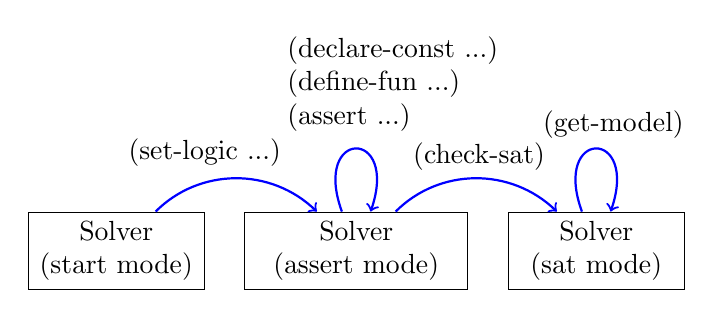
\begin{tikzpicture}
\node[rectangle, draw, align=center, text width=2cm] (a) {Solver\\(start mode)};
\node[align=left, above=4.5mm of a.north east] (in1) {(set-logic ...)};

\node[rectangle, draw, align=center, text width=2.6cm] (b) [right=5mm of a] {Solver\\(assert mode)};
\node at (b) [align=left, above right = 14mm and -10mm] (in2) {(declare-const ...)\\(define-fun ...)\\(assert ...)};

\node at (b) [align=left, above right=9mm and 6mm] (in2) {(check-sat)};

\node[rectangle, draw, align=center, text width=2cm, ] (c) [right=5mm of b] {Solver\\(sat mode)};
\node at (c) [align=left, above right=13mm and -8mm] (in2) {(get-model)};
% https://tikz.dev/tikz-arrows#sec-16.3.3
\draw [draw = blue, thick,
arrows={
	-> [bend,]}]
(a) edge [bend left=45] (b)
(b) edge [in=70, out=110,looseness=8] (b)
(b) edge [bend left=45] (c)
(c) edge [in=70, out=110,looseness=8] (c);

\end{tikzpicture}
	\caption{A simple interaction with an SMT-LIB standard solver. If the formula \texttt{assert}ed in assert mode was unsatisfiable, the solver would instead enter unsat mode and a different set of commands would be valid.}
	\label{fig:smt-lib}
\end{figure}

For a full description of SMT-LIB, readers are referred to \cite{smtlib2}. As the purpose of our software is to provide an abstraction on top of SMT-LIB, we refrain from an in-depth description of the language. Knowledge of SMT-LIB is not required to understand and use the basic functionality of \verb|BooleanSatisfiability.jl|.

In this section we make use of Julia's type notation \verb|f(x::Type)| to disambiguate the types of function arguments when necessary.

\section{Package Design}

Our software facilitates the construction and SMT-LIB representation of SMT formulae, along with providing a simple interface to SMT-LIB compliant theorem provers.

The basic unit of a formula in our software is the expression (Figure \ref{fig:expr-tree}).

\begin{figure}[h]
	\centering
		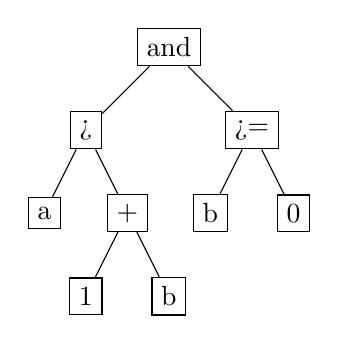
\begin{tikzpicture}[level distance=3em,
	level 1/.style={sibling distance=6em},
	level 2/.style={sibling distance=3em}]
	\node[rectangle, draw] {and}
	child {node[rectangle, draw] {>}
		child{node[rectangle, draw] {a}}
		child{node[rectangle, draw] {+}
			child{node[rectangle, draw] {1}}
			child{node[rectangle, draw] {b}}
		}
	}
	child {node[rectangle, draw] {>=}
		child {node[rectangle, draw] {b}}
		child {node[rectangle, draw] {0}}
	};
	\end{tikzpicture}
	\caption{The expression \texttt{and(a > b + 1, b >= 0)}.}
	\label{fig:expr-tree}
\end{figure}

Expressions may represent single variables or operators combining expressions. An abstract type \verb|AbstractExpr| is provided. Concrete types inheriting from \verb|AbstractExpr| implement a tree structure capable of representing arbitrarily complex nested expressions. Julia's type system prevents expressions from being incorrectly combined operators. For example, $\neg\verb|x|$ is only valid if \verb|x| is of type \verb|BoolExpr|.

Output types of operations follow type compatibility and promotion rules; for example, if \verb|x| is a \verb|BoolExpr| and \verb|a| is an \verb|IntExpr|, \verb|x + a| is an \verb|IntExpr|.

\subsection{Expressions}
Variables are declared using \verb|@satvariable|. Vector- and matrix-valued variables are arrays of single-valued expressions; thus, Julia's built in array functionality allows operators to be broadcast across said variables.

Elements of vector and matrix expressions are assigned human-readable names of the form \verb|name_i_j|.
\begin{verbatim}
@satvariable(x[1:2], Bool)
# x is an array of BoolExprs
# with names x_1, x_2

@satvariable(y[1:2, 1:3], Bool)
# y is an array of BoolExprs
# with names y_1_1, y_1_2, ... y_2_3 
\end{verbatim}

Expressions constructed from operators and variables take names of the format \verb|OP_HASH| where \verb|OP| is the operator name and \verb|HASH| is computed from the names of child expressions using Julia's deterministic hash function. This ensures all expressions have unique names and allows components of nested expressions to be re-used when generating the SMT-LIB representation of an expression. In future versions of our software, this could also allow for optimization by memoizing large expressions with repeated smaller components.

Expressions are simplified where possible: specifically, \verb|not(not(expr))| simplifies to \verb|expr|, and nested conjunctions or disjunctions are flattened.

\subsection{Constants}
Constants are automatically wrapped. Julia's native \verb|Bool|, \verb|Int|, and \verb|Float64| types interoperate with our \verb|BoolExpr|, \verb|IntExpr| and \verb|RealExpr| types as expected, following type promotion rules.

Numeric constants are combined when possible: for example, \verb|true + 2| will be stored as integer \verb|3| and \verb|1 + 2.5| is promoted to \verb|3.5|. Logical expressions involving constants can often be simplified. The following examples are provided.
\begin{verbatim}
@satvariable(z, Bool)
and(false, z) # returns false
implies(false, z) # returns true
iff(z, false) # returns not(z)
\end{verbatim}

\subsection{SMT-LIB representation}

While SMT-LIB permits expressions of arbitrary complexity, our software limits the depth of nested expressions by generating sub-expressions using SMT-LIB's \verb|(define-fun)| to define sub-expressions without \verb|assert|ing them. % TODO clean up this part
A representative example is provided below, with hashed names shortened for readability.
\begin{verbatim}
@satvariable(x, Bool)
@satvariable(y, Bool)
expr = or(¬x, and(¬x, y))
print(smt(expr))
> (declare-const x Bool)
> (declare-const y Bool)
> (define-fun NOT_53b20e () Bool (not x))
> (define-fun AND_eb3b71 () Bool
    (and NOT_53b20e y))
> (define-fun OR_90de3d
    () Bool (or AND_eb3b71 NOT_53b20e))
> (assert OR_90de3d)
\end{verbatim}
Note that although \verb|not(x)| appears twice in \verb|expr|, it is defined once and reused.

\subsection{Interacting with Solvers}
Internally, our package uses Julia's \verb|Process| library to interact with a solver via input and output pipes. This supports the interactive nature of SMT-LIB, which necessitates a two-way connection with the solver.
%TODO diagram of this process thing
This design provides several benefits. By transparently documenting how our software manages sessions with solvers, we eliminate many of the difficulties that arise when calling software dependencies. The process to make solvers available for \verb|BooleanSatisfiability.jl| on any system is fundamentally the same: the user must install the solver and ensure it can be invoked from their machine's command line. Users can customize the command used to invoke a solver. This provides a single mechanism for interacting with SMT-LIB compatible solvers that aren't explicitly supported; customizing options using command line flags; and working around machine-specific issues such as a solver being available under a different name or at a specific path.

\section{Using The Package}
\subsection{Working with formulae}.
The function \verb|smt(e::AbstractExpr)| returns the SMT-LIB representation of expression \verb|e| as a string. If \verb|e| is a Boolean expression, \verb|smt| will assert \verb|e|; otherwise \verb|smt| will simply generate the SMT-LIB statements defining \verb|e|. This behavior can be controlled using the optional keyword argument \texttt{assert=true|false}. The related function \verb|save(e::AbstractExpr, filename="out")| writes the output of \verb|smt(e)| to the text file \verb|out.smt|.

The function \verb|sat!(e::BoolExpr, solver::solver)| calls the given solver on \verb|e| and returns either \verb|:SAT|, \verb|:UNSAT|, or \verb|:ERROR|. If \verb|e| is \verb|:SAT|, the values of all nested expressions in \verb|e| are updated to allow easy retrieval of the satisfying assignment. If \verb|e| is \verb|:UNSAT|, the values of all nested expressions are set to \verb|nothing|.

Note that \verb|sat!| can only be called on Boolean expressions, because the purpose of a theorem prover is to determine whether a Boolean statement is \verb|true| or \verb|false|. In comparison, one can generate the SMT-LIB representation of any \verb|AbstractExpr|, including non-Boolean expressions that do not represent valid SMT problems. Tables \ref{tab:bool_ops} and \ref{tab:arithmetic_ops} provide an overview of which operators return Boolean expressions.

\section{Specifying an SMT Problem}
\subsection{Variables}
New variables are declared using the \verb|@satvariable| macro, which behaves similarly to the \verb|@variable| macro in JuMP \cite{Lubin2023}.
The \verb|@satvariable| macro takes two arguments: a variable name with optional size and shape (for creating vector-valued and matrix-valued variables), and the variable type.

\begin{verbatim}
# Single BoolExpr
@satvariable(x, Bool)

# n-vector of BoolExpr
@satvariable(y[1:n], Bool)

# m x n vector of IntExpr
@satvariable(z[1:n], Int)
\end{verbatim}
  
Variables may be combined using operations, which we distinguish by return type.
Boolean operations \verb|and|, \verb|or|, \verb|not|, \verb|xor|, \verb|implies|, \verb|iff|, and \verb|ite| (if-then-else) return Boolean expressions.


\subsection{Type Promotion}
Integer or real-valued operations \verb|+|, \verb|-|, \verb|*| return integer or real expressions using Julia type promotion rules. Division (\verb|/|) is only valid over real-valued expressions\footnote{Readers familiar with gradient-based or iterative optimization over real-valued variables should be aware that although SMT provides mechanisms to represent arithmetic over real values, decision procedures for the theory of real arithmetic are incomplete and often require an impractical amount of computation time. SMT is primarily used for representing problems involving discrete-valued variables and logical statements over said variables.
}.
\begin{verbatim}
@satvariable(a, Bool)
@satvariable(b, Int)
@satvariable(c, Real)

a + b # returns IntExpr
b + c # returns RealExpr
a + b > 1 # returns BoolExpr
\end{verbatim}

Type promotion also applies to constants. Continuing the above example:
\begin{verbatim}
b + true # IntExpr + Bool returns IntExpr
b + 1.0 # IntExpr + Real returns RealExpr
c + 1 # RealExpr + Int returns RealExpr
\end{verbatim}

\subsection{Operators}
We define the following operators.
\begin{table}[h!]
	\centering
	\begin{tabular}{|c|c|c|c|c|}
	%\hline
	%\multicolumn{5}{1}{Boolean Operators}\\
	\hline
	Operator & \# Inputs & Input Type(s) & Return Type & Symbol\\
	\hline
	\verb|or| & $n\geq 2$ & \verb|BoolExpr| & \verb|BoolExpr| & \verb|any|, \verb|∨|\\
	\hline
	\verb|and| & $n\geq 2$ & \verb|BoolExpr| & \verb|BoolExpr| & \verb|all|, \verb|∧|\\
	\hline
	\verb|not| & 1 & \verb|BoolExpr| & \verb|BoolExpr| & \verb|¬|\\
	\hline
	\verb|implies| & 2 & \verb|BoolExpr| & \verb|BoolExpr| & \verb|⟹|\\
	\hline
	\verb|xor| & $n\geq 2$ & \verb|BoolExpr| & \verb|BoolExpr| & \verb|⊻|\\
	\hline
	\verb|iff| & 2 & \verb|BoolExpr| & \verb|BoolExpr| & \verb|⟺|\\
	\hline
	\verb|ite|\tablefootnote{The operator \texttt{ite} refers to ``if-then-else". \texttt{ite(x, y, z)} is equivalent to \texttt{(x ⟹ y) ∧ (¬x ⟹ z)}.}
	& 3 & \verb|BoolExpr| & \verb|BoolExpr| & ~\\
	\hline
	\end{tabular}
\caption{Boolean operators.}
\label{tab:bool_ops}
\end{table}

\begin{table}[h!]
	\centering
	\begin{tabular}{|c|c|c|c|}
	%\hline
	%\multicolumn{5}{|1|}{Arithmetic Operators}\\
	\hline
	Operator & Input Type(s) & Return Type\\
	\hline
	\verb|>| & Any numeric expr. & \verb|BoolExpr| \\
	\hline
	\verb|>=| & Any numeric expr. & \verb|BoolExpr| \\
	\hline
	\verb|<| & Any numeric expr. & \verb|BoolExpr| \\
	\hline
	\verb|<=| & Any numeric expr. & \verb|BoolExpr| \\
	\hline
	\verb|==|\tablefootnote{To check whether two \texttt{AbstractExpr} are equivalent, use \texttt{isequal}.}
	& Any numeric expr. & \verb|BoolExpr| \\
	\hline
	\verb|-| (unary) & \verb|IntExpr|, \verb|RealExpr| & \verb|IntExpr|, \verb|RealExpr|\\
	\hline
	\verb|+| & Any numeric expr. & \verb|IntExpr|, \verb|RealExpr| \\
	\hline
	\verb|-| & Any numeric expr.& \verb|IntExpr|, \verb|RealExpr| \\
	\hline
	\verb|*| & Any numeric expr. & \verb|IntExpr|, \verb|RealExpr| \\
	\hline
	\verb|/| & \verb|RealExpr|& \verb|RealExpr| \\
	\hline
\end{tabular}
\caption{Comparison and arithmetic operators. Where ``Any numeric expr" is listed, this refers to \texttt{BoolExpr}, \texttt{IntExpr}, \texttt{RealExpr}, or a \texttt{Bool}, \texttt{Int}, or \texttt{Float} constant. The return type of an arithmetic operator is determined by Julia's \texttt{Int} and \texttt{Float} type promotion rules.}
\label{tab:arithmetic_ops}
\end{table}

\subsection{Operator Precedence}
Julia defines the operator precedence and associativity for all symbolic operators defined in this package.
For the most up-to-date description of Julia's operator precedence rules, see \cite{Julia_documentation_2023}.
One can also determine operator precedence using the call \verb|Base.operator_precedence(s)| where \verb|s| is a symbol (e.g. \verb|:+| or \verb|:*|). Higher numbers indicate greater precedence.

Precedence and associativity rules can yield misleading expressions or unexpected type errors. Readers are encouraged to parenthesize expressions, avoiding potential sources of confusion. The following illustrative examples are provided.

\begin{verbatim}
@satvariable(x, Bool)
@satvariable(y, Bool)
@satvariable(z, Bool)

x⟹y ∧ y⟹z
# this is implies(x, implies(and(y, y), z))
# it is not (x⟹y) ∧ (y⟹z)

x ∧ y + z # equivalent to (x ∧ y) + z

@satvariable(a, Int)
@satvariable(b, Int)

a >= 1 ∨ b >= 1 # yields a type error
(a >= 1) ∨ (b >= 1) # valid expression
\end{verbatim}

\section{Examples}
% TODO

\subsection*{Custom solver interactions}
We expose the low-level interface, allowing advanced users to send SMT commands and receive prover responses. Users are responsible for ensuring the correctness of these commands, as well as interpreting the results. In this use case, \verb|BooleanSatisfiability.jl| can be used to automate generation of the SMT problem and programmatically interact with solvers, extending the usability of the SMT interface.

\section{Conclusions}
We have successfully developed a Julia package providing a simple, high-level interface to SMT-LIB compatible solvers. Our package takes advantage of Julia's functionality to construct a simple and extensible interface; we use multiple dispatch to optimize and simplify operations over constants, the type system to enforce the correctness of SMT expressions, and \verb|Base.Process| to interact with SMT-LIB solvers.

\section{Acknowledgements}
The software architecture of \verb|BooleanSatisfiability.jl| was inspired by \verb|Convex.jl|, \verb|JuMP|, and \verb|PySMT| \cite{convexjl, Lubin2023, pysmt2015}. Ideas, suggestions and feedback on the package's user interface were provided by Prof. Mykel Kochenderfer.

\section{Future Work}

\printbibliography


%\subsection{Maintaining the Integrity of the Specifications}

%\subsection{Abbreviations and Acronyms}\label{AA}
%Define abbreviations and acronyms the first time they are used in the text, 
%even after they have been defined in the abstract. Abbreviations such as 
%IEEE, SI, MKS, CGS, ac, dc, and rms do not have to be defined. Do not use 
%abbreviations in the title or heads unless they are unavoidable.

%\subsection{Equations}
%Number equations consecutively. To make your 
%equations more compact, you may use the solidus (~/~), the exp function, or 
%appropriate exponents. Italicize Roman symbols for quantities and variables, 
%but not Greek symbols. Use a long dash rather than a hyphen for a minus 
%sign. Punctuate equations with commas or periods when they are part of a 
%sentence, as in:
%\begin{equation}
%a+b=\gamma\label{eq}
%\end{equation}

%Be sure that the 
%symbols in your equation have been defined before or immediately following 
%the equation. Use ``\eqref{eq}'', not ``Eq.~\eqref{eq}'' or ``equation \eqref{eq}'', except at 
%the beginning of a sentence: ``Equation \eqref{eq} is . . .''

%\subsection{\LaTeX-Specific Advice}

%Please note that the \verb|{subequations}| environment in {\LaTeX}
%will increment the main equation counter even when there are no
%equation numbers displayed. If you forget that, you might write an
%article in which the equation numbers skip from (17) to (20), causing
%the copy editors to wonder if you've discovered a new method of
%counting.

%{\BibTeX} does not work by magic. It doesn't get the bibliographic
%data from thin air but from .bib files. If you use {\BibTeX} to produce a
%bibliography you must send the .bib files. 

%{\LaTeX} can't read your mind. If you assign the same label to a
%subsubsection and a table, you might find that Table I has been cross
%referenced as Table IV-B3. 

%{\LaTeX} does not have precognitive abilities. If you put a
%\verb|\label| command before the command that updates the counter it's
%supposed to be using, the label will pick up the last counter to be
%cross referenced instead. In particular, a \verb|\label| command
%should not go before the caption of a figure or a table.

%Do not use \verb|\nonumber| inside the \verb|{array}| environment. It
%will not stop equation numbers inside \verb|{array}| (there won't be
%any anyway) and it might stop a wanted equation number in the
%surrounding equation.

%\subsection{Some Common Mistakes}\label{SCM}
%\begin{itemize}
%\item The word ``data'' is plural, not singular.
%\item The subscript for the permeability of vacuum $\mu_{0}$, and other common scientific constants, is zero with subscript formatting, not a lowercase letter ``o''.
%\item In American English, commas, semicolons, periods, question and exclamation marks are located within quotation marks only when a complete thought or name is cited, such as a title or full quotation. When quotation marks are used, instead of a bold or italic typeface, to highlight a word or phrase, punctuation should appear outside of the quotation marks. A parenthetical phrase or statement at the end of a sentence is punctuated outside of the closing parenthesis (like this). (A parenthetical sentence is punctuated within the parentheses.)
%\item A graph within a graph is an ``inset'', not an ``insert''. The word alternatively is preferred to the word ``alternately'' (unless you really mean something that alternates).
%\item Do not use the word ``essentially'' to mean ``approximately'' or ``effectively''.
%\item In your paper title, if the words ``that uses'' can accurately replace the word ``using'', capitalize the ``u''; if not, keep using lower-cased.
%\item Be aware of the different meanings of the homophones ``affect'' and ``effect'', ``complement'' and ``compliment'', ``discreet'' and ``discrete'', ``principal'' and ``principle''.
%\item Do not confuse ``imply'' and ``infer''.
%\item The prefix ``non'' is not a word; it should be joined to the word it modifies, usually without a hyphen.
%\item There is no period after the ``et'' in the Latin abbreviation ``et al.''.
%\item The abbreviation ``i.e.'' means ``that is'', and the abbreviation ``e.g.'' means ``for example''.
%\end{itemize}
%An excellent style manual for science writers is \cite{b7}.


%\subsection{Identify the Headings}
%Headings, or heads, are organizational devices that guide the reader through 
%your paper. There are two types: component heads and text heads.
%
%Component heads identify the different components of your paper and are not 
%topically subordinate to each other. Examples include Acknowledgments and 
%References and, for these, the correct style to use is ``Heading 5''. Use 
%``figure caption'' for your Figure captions, and ``table head'' for your 
%table title. Run-in heads, such as ``Abstract'', will require you to apply a 
%style (in this case, italic) in addition to the style provided by the drop 
%down menu to differentiate the head from the text.
%
%Text heads organize the topics on a relational, hierarchical basis. For 
%example, the paper title is the primary text head because all subsequent 
%material relates and elaborates on this one topic. If there are two or more 
%sub-topics, the next level head (uppercase Roman numerals) should be used 
%and, conversely, if there are not at least two sub-topics, then no subheads 
%should be introduced.
%
%\subsection{Figures and Tables}
%\paragraph{Positioning Figures and Tables} Place figures and tables at the top and 
%bottom of columns. Avoid placing them in the middle of columns. Large 
%figures and tables may span across both columns. Figure captions should be 
%below the figures; table heads should appear above the tables. Insert 
%figures and tables after they are cited in the text. Use the abbreviation 
%``Fig.~\ref{fig}'', even at the beginning of a sentence.
%
%\begin{table}[htbp]
%\caption{Table Type Styles}
%\begin{center}
%\begin{tabular}{|c|c|c|c|}
%\hline
%\textbf{Table}&\multicolumn{3}{|c|}{\textbf{Table Column Head}} \\
%\cline{2-4} 
%\textbf{Head} & \textbf{\textit{Table column subhead}}& \textbf{\textit{Subhead}}& \textbf{\textit{Subhead}} \\
%\hline
%copy& More table copy$^{\mathrm{a}}$& &  \\
%\hline
%\multicolumn{4}{l}{$^{\mathrm{a}}$Sample of a Table footnote.}
%\end{tabular}
%\label{tab1}
%\end{center}
%\end{table}
%
%\begin{figure}[htbp]
%\centerline{\includegraphics{fig1.png}}
%\caption{Example of a figure caption.}
%\label{fig}
%\end{figure}
%
%Figure Labels: Use 8 point Times New Roman for Figure labels. Use words 
%rather than symbols or abbreviations when writing Figure axis labels to 
%avoid confusing the reader. As an example, write the quantity 
%``Magnetization'', or ``Magnetization, M'', not just ``M''. If including 
%units in the label, present them within parentheses. Do not label axes only 
%with units. In the example, write ``Magnetization (A/m)'' or ``Magnetization 
%\{A[m(1)]\}'', not just ``A/m''. Do not label axes with a ratio of 
%quantities and units. For example, write ``Temperature (K)'', not 
%``Temperature/K''.
%
%\section*{Acknowledgment}
%
%The preferred spelling of the word ``acknowledgment'' in America is without 
%an ``e'' after the ``g''. Avoid the stilted expression ``one of us (R. B. 
%G.) thanks $\ldots$''. Instead, try ``R. B. G. thanks$\ldots$''. Put sponsor 
%acknowledgments in the unnumbered footnote on the first page.
%
%\section*{References}
%
%Please number citations consecutively within brackets \cite{b1}. The 
%sentence punctuation follows the bracket \cite{b2}. Refer simply to the reference 
%number, as in \cite{b3}---do not use ``Ref. \cite{b3}'' or ``reference \cite{b3}'' except at 
%the beginning of a sentence: ``Reference \cite{b3} was the first $\ldots$''
%
%Number footnotes separately in superscripts. Place the actual footnote at 
%the bottom of the column in which it was cited. Do not put footnotes in the 
%abstract or reference list. Use letters for table footnotes.
%
%Unless there are six authors or more give all authors' names; do not use 
%``et al.''. Papers that have not been published, even if they have been 
%submitted for publication, should be cited as ``unpublished'' \cite{b4}. Papers 
%that have been accepted for publication should be cited as ``in press'' \cite{b5}. 
%Capitalize only the first word in a paper title, except for proper nouns and 
%element symbols.
%
%For papers published in translation journals, please give the English 
%citation first, followed by the original foreign-language citation \cite{b6}.
%
%\begin{thebibliography}{00}
%\bibitem{b1} G. Eason, B. Noble, and I. N. Sneddon, ``On certain integrals of Lipschitz-Hankel type involving products of Bessel functions,'' Phil. Trans. Roy. Soc. London, vol. A247, pp. 529--551, April 1955.
%\bibitem{b2} J. Clerk Maxwell, A Treatise on Electricity and Magnetism, 3rd ed., vol. 2. Oxford: Clarendon, 1892, pp.68--73.
%\bibitem{b3} I. S. Jacobs and C. P. Bean, ``Fine particles, thin films and exchange anisotropy,'' in Magnetism, vol. III, G. T. Rado and H. Suhl, Eds. New York: Academic, 1963, pp. 271--350.
%\bibitem{b4} K. Elissa, ``Title of paper if known,'' unpublished.
%\bibitem{b5} R. Nicole, ``Title of paper with only first word capitalized,'' J. Name Stand. Abbrev., in press.
%\bibitem{b6} Y. Yorozu, M. Hirano, K. Oka, and Y. Tagawa, ``Electron spectroscopy studies on magneto-optical media and plastic substrate interface,'' IEEE Transl. J. Magn. Japan, vol. 2, pp. 740--741, August 1987 [Digests 9th Annual Conf. Magnetics Japan, p. 301, 1982].
%\bibitem{b7} M. Young, The Technical Writer's Handbook. Mill Valley, CA: University Science, 1989.
%\end{thebibliography}
%\vspace{12pt}
%\color{red}
%IEEE conference templates contain guidance text for composing and formatting conference papers. Please ensure that all template text is removed from your conference paper prior to submission to the conference. Failure to remove the template text from your paper may result in your paper not being published.

\end{document}
